\section{Information Security}

The basic building stones of information security are confidentiality, integrity and availability, also called the \textit{"CIA - triad"} \cite{stallings}.
\textbf{Confidentiality} is used to protect sensitive information from eavesdroppers who are not allowed to get knowledge of that information. 
\textbf{Integrity} ensures that some kind of information can not be altered by third-parties, or that such a modification can be detected by the
receiver of the information, and also includes information non-repudiation.
\textbf{Availability} ensures that information, which is needed by an entity to provide some service, is accessible.
\\
All three properties go hand-in-hand with each other because a successful attack on one property may allow attacking another one. For example, if a
confidentiality attack against a computer system responsible for money transfers can be conducted to steal a password used for controlling this system,
an attacker
can subsequently render the system unusable, therefore compromising availability. On the other hand, the attacker could also try to remain undetected and change
booking orders, thus mounting an attack against the integrity of the system. Thus, these 3 basic concepts are interleaved, and building a system which honors
only parts of them will most likely lead to an insecure system.
\\
\\
A basic classification of attacks is given in figure \ref{fig:attacks} - a refinement will be given in this work as additional attacks are introduced.
The most abstract level distinguishes \textit{passive} and \textit{active} attacks. A passive
attack is undetectable and aimed against confidentiality, either to release the data itself or to get knowledge of some kind of meta data, like origin,
destination and frequency of a data flow - to counter them, encryption is sufficient. Passive attacks are often used as starting point for obtaining knowledge which can later to be used to mount 
additional attacks.
\\
Unfortunately, a restriction to passive attacks only is not realistic for many systems. Whenever the adversary has access to the communication medium, active attacks
cannot be ruled out. A replay attack happens when the attacker monitors traffic first (i.e. a passive attack) and afterwards injects a recorded package, 
attacking data freshness. Of course,
the package can also be modified and injected afterwards.
A \gls{dos} attack tries to overload system resources, attacking availability s.t. the system is not
usable by legitimate users. Finally, masquerade attacks turn on the integrity of the system.
\begin{figure}
    \centering
    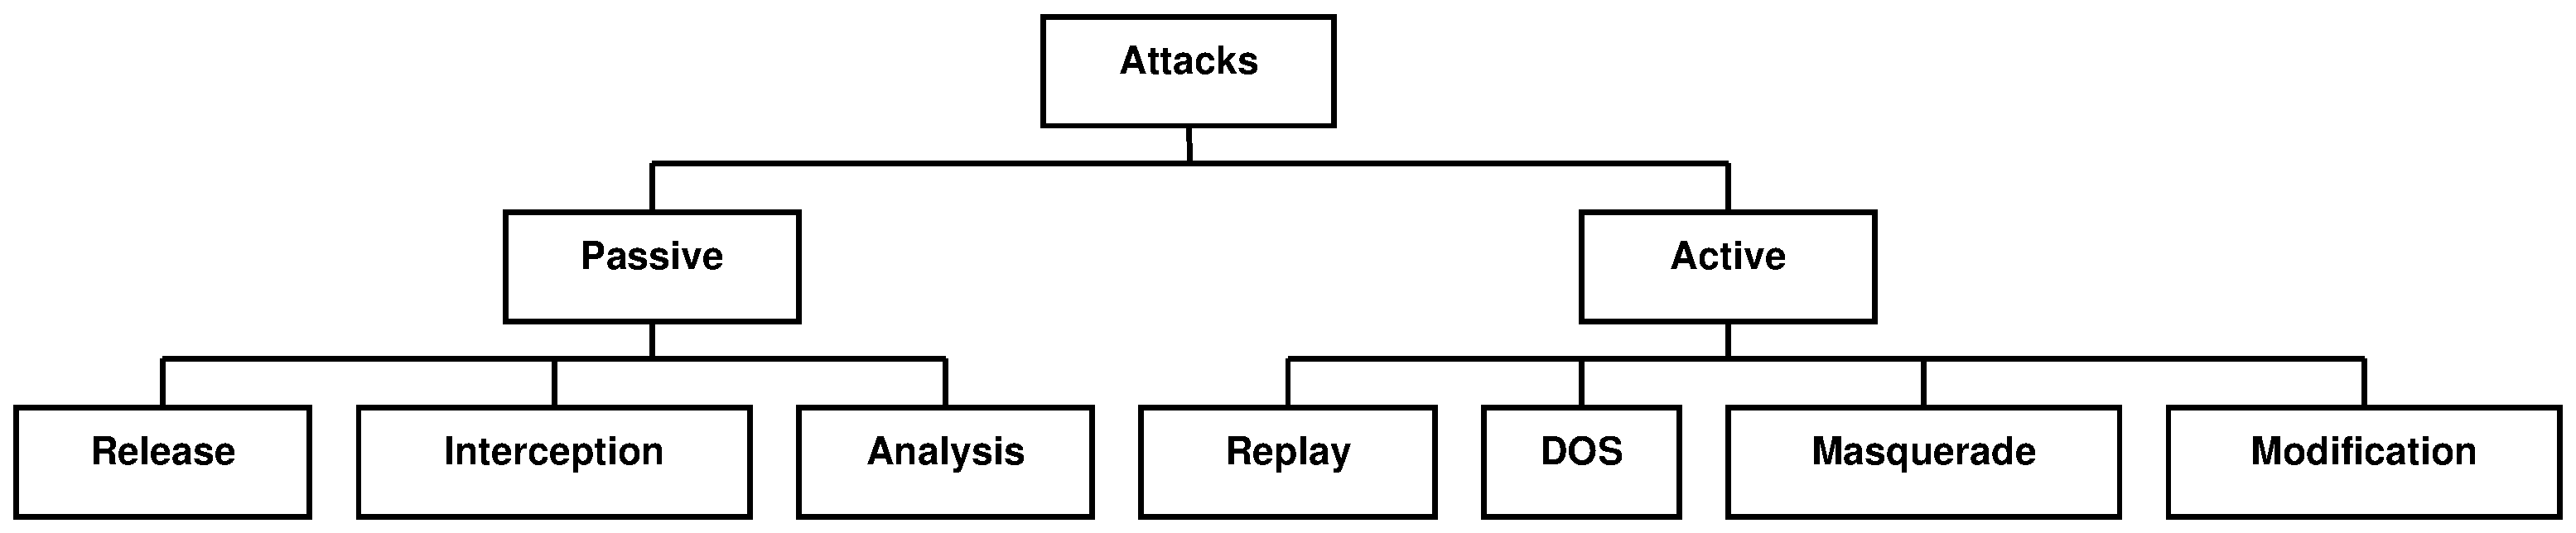
\includegraphics[width=1\textwidth]{figures/attacks.eps}
    \caption{Classification of attacks}
    \label{fig:attacks}
\end{figure}
\\
\\
The basic tool to achieve information security is cryptography, which is introduced in the following sections. Improved availability, with established 
information security measurements as necessary, but not sufficient prerequisites, is gained through replication, presented afterwards.
Finally, the special requirements that must be met for \gls{hba} will be researched in this chapter.

%Additionally to the CIA - triad, sometimes two more concepts are used in the security field: \textbf{Authenticity} is tied to integrity and ensures the property
%of being genuine, while \textbf{Accountability} allows to link actions performed on a system uniquely to the entity responsible for them.
